\section{Résultats obtenus}
	L'application permet de personnaliser la position de la sortie. Le placement des obstacles à l'intérieur de la pièce correspond aux dispositions des tables dans une salle de classe. Une interface est fournie pour permettre cette personnalisation : Figure~\ref{fig:distances_parcourues}
		
	\begin{figure}[!H]
	\centering
	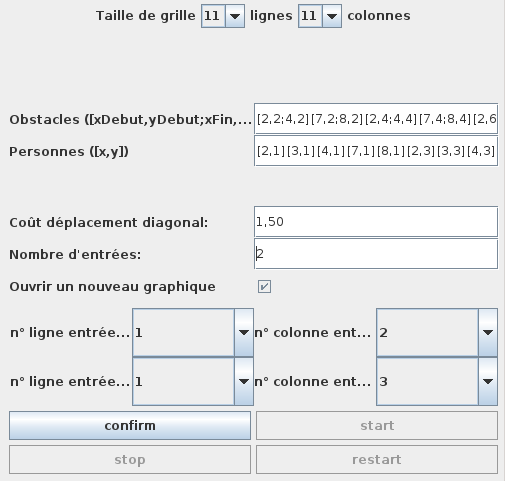
\includegraphics[scale=0.7]{imagesPNG/personnalisation.png}
	\caption{Représentation des distances parcourues\label{fig:distances_parcourues}}
	\end{figure}
		
	Une fois cette personnalisation effectuée et validée, la grille est générée, et les fenêtres contenant les diagrammes s'ouvrent en parallèle. L'utilisateur n'a plus qu'à cliqué sur le boutons "Start" pour démarrer la simulation de l'évacuation. Cette dernière continuera jusqu'à ce que l'évacuation soit complète, en mettant à jour les diagrammes en temps réel. Cependant, l'utilisateur a la possibilité de stopper la simulation grâce au bouton "Stop".
		
	\textbf{SCREENSHOT}